\graphicspath{{chapters/01_abstract/images}}
\chapter*{Abstract}
\addcontentsline{toc}{chapter}{Abstract}

% The Abstract is a short summary, usually about 1 page in length, that provides the context and the objectives of the project, and summarizes the scientific problem, the techniques used and the results obtained. In case of collaborative work, here is where the graduating student gives details on his or her contribution to the study. Full document should have a maximum of 85 pages, excluding reference list and any appendices.

% TODO: Create graphical abstract
\begin{figure}[h]
  \centering
  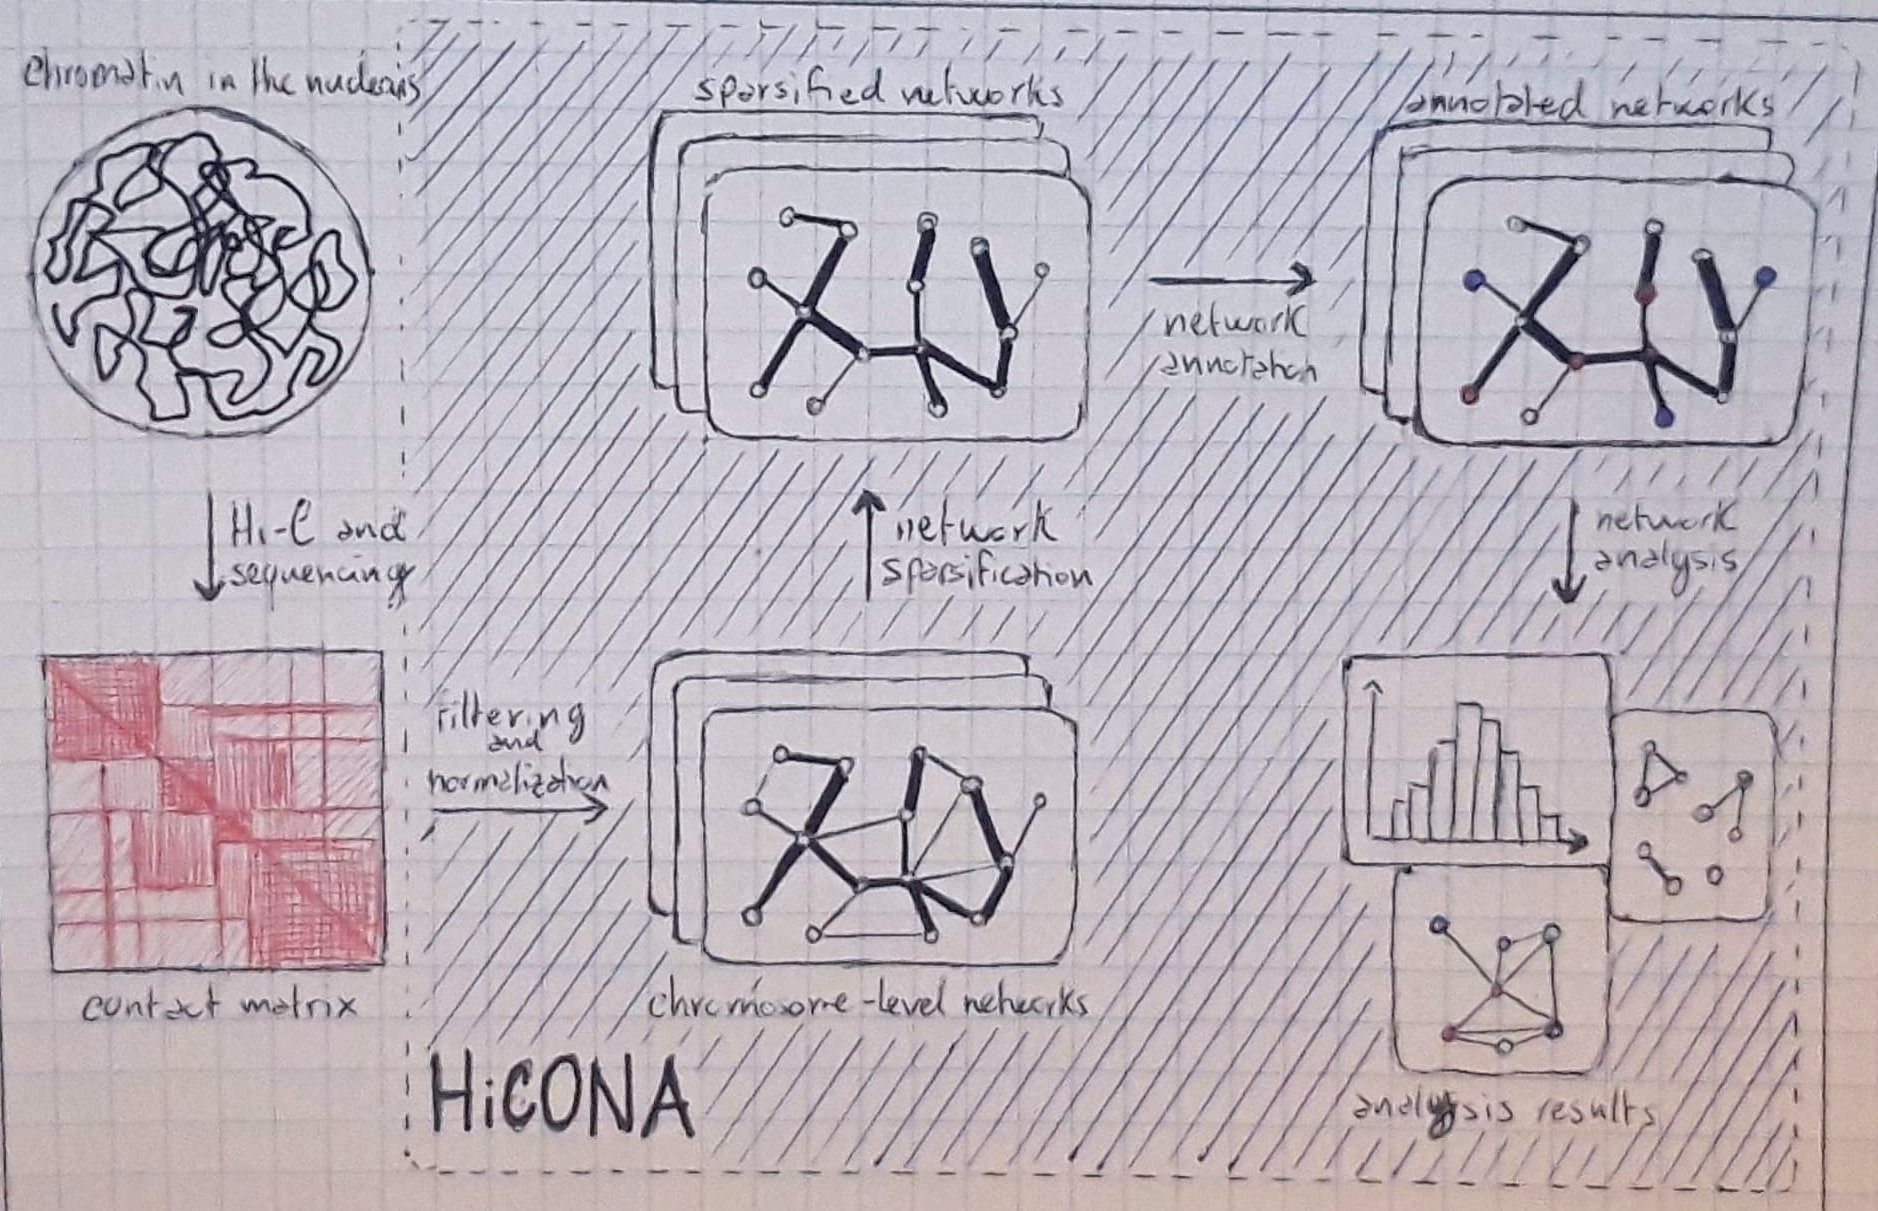
\includegraphics[width=1\textwidth]{graphical_abstract.jpeg}
\end{figure}

The usage of network analysis to study chromatin organization is still at a nascent stage; while there exist some network analysis-based tools or procedures which use network analysis algorithms, their applications are generally restricted to a very narrow set of capabilities and can hardly ever be used for purposes different from the main one for which they were designed. Still, network analysis could provide major insights into chromatin organization; it is thus of great importance to develop the means necessary to easily conduct this type of analysis. For this reason, during my internship, I took part in the design and implementation proccess of HiCONA, a Python3 package aimed at providing a flexible framework in order to conduct any type of network analysis on data coming from Hi-C experiments (a chromosome conformation capture technique). The package provides functionalities to preprocess Hi-C data, which entails filtering, normalization and network sparsification; the data is then used to create graphs, which can be annotated and analysed using algorithms from standard network analysis, which were taylored to Hi-C data derived networks. Keeping into account user-friendliness, the package was optimized in order to be able to process almost any Hi-C data file even on less performing systems, such as laptops. In this thesis, the main focus will be on the preprocessing part of the package, how it was implemented and how it performs, both in terms of computational efficiency as well as reproducibility and consistency. Some network analysis operations which can be conducted using the package will also be discussed, though briefly since that they are still under developement.
